\chapter{Sagittarius A* Calibration and Parameter Sweeps}
\label{ch:calib}

\section{From simulation units to the sky}
\label{sec:conversion}

The \sgra{} calibration adopts the GRAVITY mass and distance
\citep{Gravity2022} and the EHT viewing geometry
\citep[$i \approx 30\degr$;][]{EHT2022}. The conversion from the traced
boundary to a sky angle proceeds step by step as follows
(\texttt{sweep\_tool calibrate}).
\begin{enumerate}
\item One gravitational radius is
$R_g = GM/c^2 = 4.297\times10^{6} \times 1.4766\,\mathrm{km}
     = 6.346\times10^{9}\,\mathrm{m}$,
using $GM_\odot/c^2 = 1.4766$~km.
\item At $D = 8277\,\mathrm{pc} = 2.554\times10^{20}$~m it subtends
$\theta_g = R_g/D = 2.485\times10^{-11}\,\mathrm{rad}
 = \UasPerM\,\muas$.
\item The traced critical boundary at $\astar = 0.94$, $i = 30\degr$ has
mean diameter $\CalDiamM\,M$ (32-direction average of the bisected
boundary, converted to impact parameters).
\item The photon-ring angular diameter is therefore
$d_{\rm ring} = \CalDiamM \times \UasPerM = \CalDiamUas\,\muas$.
\end{enumerate}
This falls within the EHT ring measurement of $51.8\pm2.3\,\muas$ and the
inferred shadow diameter of $48.7\pm7\,\muas$ \citep{EHT2022}. At this
near-face-on inclination the shadow is nearly circular (axis ratio
\CalAxisRatio), consistent with the weak spin dependence emphasised by
\citet{Psaltis2016}.

\section{Error budget}
\label{sec:errorbudget}

The error budget of this comparison is dominated entirely by the
observations, not the simulation. The traced boundary is bisected to
$\sim$$10^{-9}$~rad in camera angle ($\ll 10^{-3}\,\muas$ equivalent),
and the tolerance-independence established in
Chapter~\ref{ch:numerics} removes the integrator from the budget.
On the calibration side the conversion scales as
$\theta_g \propto M/D$, so
\begin{equation}
\frac{\sigma_{\theta}}{\theta}
= \sqrt{\left(\frac{\sigma_M}{M}\right)^{\!2}
+ \left(\frac{\sigma_D}{D}\right)^{\!2}}
= \sqrt{0.28^2 + 0.11^2}\,\% \simeq 0.30\,\%,
\label{eq:calibprop}
\end{equation}
about $0.15\,\muas$, twenty times smaller than the EHT error bar.
(Equation \eqref{eq:calibprop} treats the GRAVITY $M$ and $D$ as
independent; in truth they emerge correlated from the same orbit fits
— the very $M$--$R_0$ geometry of Chapter~\ref{ch:fitting} — and
since the correlation is positive, part of it cancels in the ratio
$M/D$, making \eqref{eq:calibprop} mildly conservative.) The
comparison is therefore limited by the $2.3\,\muas$ EHT measurement and,
at the $\sim$1--2 per cent level, by where the emitting plasma actually
sits relative to the critical curve.

\section{The spin--inclination plane}
\label{sec:sweep}

Fig.~\ref{fig:sweep} maps the ring diameter over the
full $(\astar, i)$ plane: at each of the $20\times20$ grid points the
complete 32-direction bisection metrology of
Chapter~\ref{ch:shadow} is repeated from scratch — four hundred
independently traced critical boundaries, every one anchored to the
same tolerance-independent machinery, with the $\astar = 0$ row
reproducing the Synge value identically at all inclinations as a
built-in control. The total spread across the physical plane is a few
per cent, illustrating the well-known spin--inclination degeneracy of
ring-size measurements: spin shrinks the mean diameter slightly,
inclination reshapes it slightly, and over most of the plane the two
effects trade against each other inside the EHT error bar.

What would break the degeneracy is worth stating, since the machinery
to predict each candidate already exists in this report. The
\emph{sub-ring} structure of Chapter~\ref{ch:ring} sharpens with
resolution rather than brightness, and its azimuthal width/flux
variation tracks the Lyapunov band of Chapter~\ref{ch:shadow}, which
\emph{does} depend on spin at fixed diameter; interferometric
detection of the $n = 1$ ring is therefore the cleanest
spin-at-fixed-size observable \citep{Johnson2020}. Independently, the
shape observables below — axis ratio and centroid displacement —
scale as $\astar\sin i$ and so separate the two parameters if imaging
fidelity ever reaches the sub-per-cent regime. Both statements are
quantitative outputs of this simulator, not aspirations.

\begin{figure}
\centering
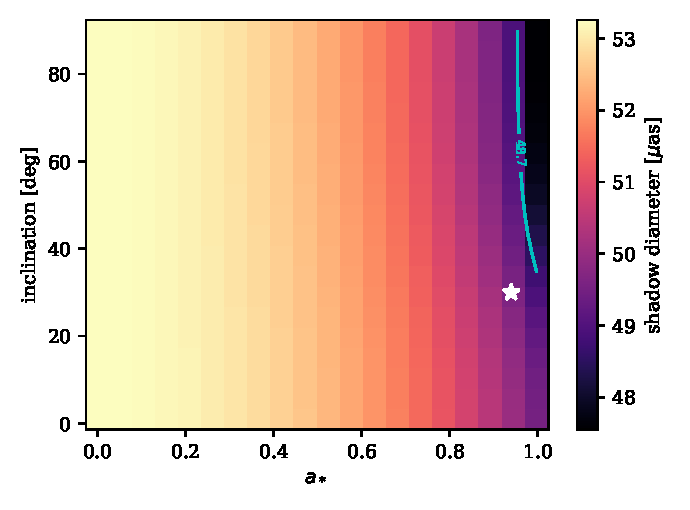
\includegraphics[width=0.7\textwidth]{figures/fig_shadow_sweep.pdf}
\caption{Photon-ring angular diameter at the GRAVITY mass and distance as a
function of spin and inclination ($20\times20$ grid of traced boundaries).
The EHT band $51.8\pm2.3\,\muas$ is indicated; the measurement constrains
the $(\astar, i)$ plane only weakly.}
\label{fig:sweep}
\end{figure}

Diameter is not the only observable the boundary carries. The extended
sweep also records the \emph{axis ratio} $d_x/d_y$ and the horizontal
\emph{centroid displacement} of the boundary
(Fig.~\ref{fig:shapemaps}) — the two shape signatures through which
spin could in principle be recovered where size cannot. Both behave as
the critical-curve geometry of Chapter~\ref{ch:shadow} predicts: the
distortions grow with $\astar \sin i$, reaching a few per cent
flattening and a displacement of $\sim 1\,M$ only in the
high-spin, near-edge-on corner. At the \sgra{} viewing geometry
($i \approx 30\degr$, white star) the axis ratio is
\CalAxisRatio{} — a fraction of a per cent from circular, far below
current imaging fidelity, which is the quantitative content of the
statement that present EHT data cannot measure \sgra's spin from the
ring shape \citep{Psaltis2016}. The shape maps also connect to the
spin-morphology discussion of Section~\ref{sec:spinmorphology}: the
displacement map is the quantitative footprint of the prograde-side
flattening visible in the renders.

\begin{figure}
\centering
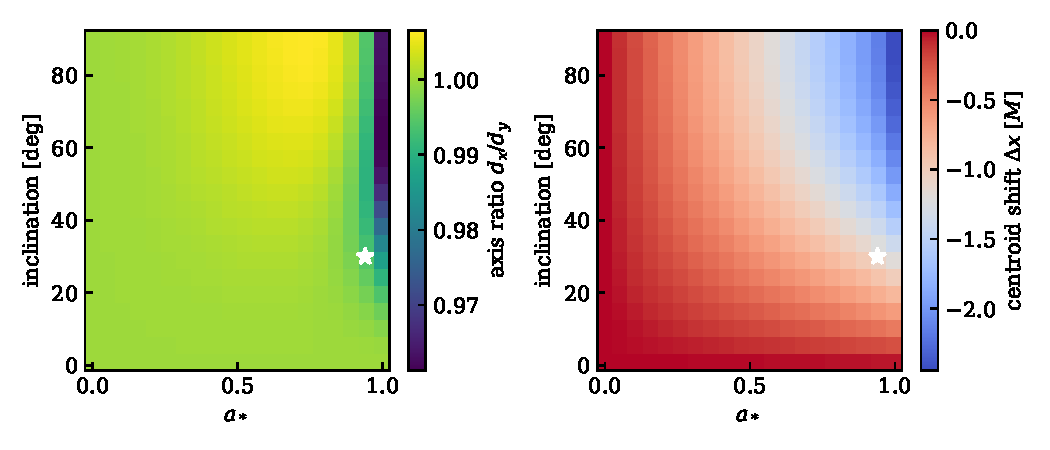
\includegraphics[width=\textwidth]{figures/fig_shadow_shape_maps.pdf}
\caption{Shape observables over the $(\astar, i)$ plane from the
extended sweep (\texttt{sweep\_tool}): boundary axis ratio (left) and
horizontal centroid displacement (right). The white star marks the
\sgra{} geometry, where both signatures are sub-per-cent.}
\label{fig:shapemaps}
\end{figure}
